% =====================================================================================
\section{Introduction}
\label{sec:intro}
% =====================================================================================

An optical phased array (OPA) splits a laser beam into coherent copies, sends each down its own waveguide and
emits each from a grating. The phase difference between neighbouring emitters sets the direction of the combined
beam across the array; the grating period and the wavelength set it along the other
axis~\cite{sun2013}. OPAs point beams without moving parts and are studied for LiDAR, free-space optical
links and biophotonic probes~\cite{hsu2022}.

In silicon the phases are usually set thermo-optically: a heater above a waveguide raises its refractive index and
delays the light. The conventional design gives each emitter its own heater and wire, and treats heat leaking to
neighbouring waveguides (thermal crosstalk) as a defect. It is suppressed by spacing the heaters
\qtyrange{15}{100}{\micro\metre} apart and converging the waveguides afterwards~\cite{phare2018,miller2020},
by trenches and undercuts~\cite{parsons2025,fang2011}, or by calibration. \Cref{fig:topview}(a) shows the result: $N$ heaters, $N$ wires and a fan-in region
whose only purpose is to keep the heaters apart.

\begin{figure}[htbp]
  \centering
  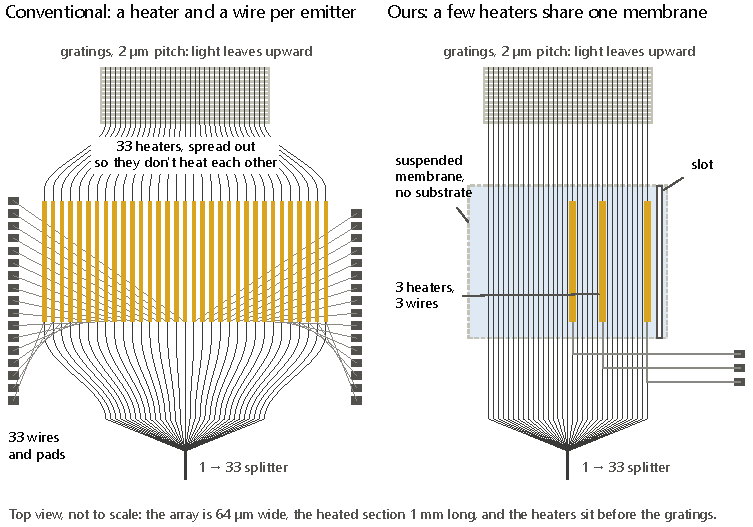
\includegraphics[width=\linewidth]{fig12_topview}
  \caption{A conventional thermo-optic OPA and the design studied here, seen from above (schematic). (a)~One
  heater, wire and pad per emitter, with the heaters spaced so that their heat does not overlap, and a fan-in to
  the emitter pitch. (b)~This work: the waveguides stay at the emitter pitch and cross a suspended oxide membrane
  before the gratings. One to three heaters set the phase of all \num{33} waveguides through the heat they share;
  a slot past the edge heater forces that heat to cross the array.}
  \label{fig:topview}
\end{figure}

Individual heaters provide three capabilities. (i)~\emph{Arbitrary patterns}: each emitter can take any phase, so
the array can form several beams or holograms. (ii)~\emph{Phase wrapping}: phase matters only modulo $2\pi$, so no
heater ever supplies more than $2\pi$. (iii)~\emph{Per-emitter calibration}: each waveguide's fabrication error can
be cancelled by its own heater.

Steering, however, needs only a smooth phase profile, a linear ramp across the array, and heat spreads smoothly.
This report therefore asks:
\begin{quote}
  With $K$ heaters driving $N>K$ emitters through shared heat, how well can the array steer and focus, and what
  does it cost in power, speed and control compared with one isolated heater per emitter?
\end{quote}

Steady heat conduction acts as a spatial low-pass filter on the phase: whatever the heaters supply is smoothed
over a spreading length $\Lth$. If $\Lth$ is shorter than the emitter pitch $d$, each heater addresses one emitter,
which is the conventional design. If $\Lth\gg d$, a few heaters reach every emitter, but only smooth profiles can
be made (an offset, a ramp, a dome). Two consequences follow immediately. A ramp cannot be wrapped, so it must be
built in full: at \ang{10} the last emitter must lead the first by \qty{45}{\rad}. And independent fabrication
errors, the sharpest pattern of all, cannot be corrected. The ratio $\Lth/d$, set by the layer structure, decides
the regime.

\paragraph{Approach.} The study is simulation only (\cref{fig:pipeline}). COMSOL finite-element models supply the
physics: the waveguide mode and its thermo-optic coefficient, the optical coupling between waveguides, the
steady and transient temperature that one heater produces at every waveguide, the grating emission, and the limit
of the linear thermal model (\cref{sec:models}). Each is checked for convergence, energy balance and consistency
(\cref{sec:verification}). Because heat conduction is linear, the phases are a matrix product of the COMSOL
profiles and the heater powers; a Python model built on this, and checked against analytic limits, searches
thousands of heater layouts (\cref{sec:methods}).

\paragraph{Main results.}
\begin{enumerate}
  \item On a standard stack, heat sinks into the substrate within \qty{3.3}{\micro\metre}, and few heaters cannot
        steer. On an oxide membrane suspended under the whole array, three to four heaters steer
        \ang{\pm 16}--\ang{22.8} at about \qty{4.9}{\mWdeg}.
  \item A slot cut past the edge heater forces all its heat to cross the array, which makes the temperature a
        straight ramp. Three heaters then steer \ang{22.8} at \qty{1.38}{\mWdeg}; in vacuum one heater does so at
        \qty{0.53}{\mWdeg}, within \qty{5}{\percent} of a conduction limit that is independent of $N$.
  \item This is \numrange{10}{30} times below published few-wire arrays. Because the ramp cannot be wrapped,
        however, \num{33} of the best published folded phase shifters would need \num{3.6} times less power at
        \ang{10}.
  \item All three capabilities of individual control are lost, and each loss is quantified: two to four usable
        phase patterns, no correction of independent fabrication errors (so a one-time trim is required), and a
        hottest waveguide about \qty{62}{\kelvin} above ambient at \ang{10}.
  \item A \ang{10} step settles in \qtyrange{2}{9}{\milli\second} with a plain step drive. Because the heaters are
        few and independent, their drives can be shaped in time (pre-emphasis), which shortens this six to
        twelve times at three times the hold power.
  \item A uniformly heated membrane between two walls has a parabolic temperature profile, so one heater forms a
        tunable cylindrical lens at about \qty{1.2}{\milli\watt\per\rad}.
\end{enumerate}

To our knowledge, this is the first design study to use lateral heat spreading from one to five heaters as the
main steering and focusing actuator, with the membrane shaped to make the profile linear (\cref{sec:related}).

\Cref{sec:background} gives the theory, \cref{sec:models,sec:methods} the models, and \cref{sec:verification} the
checks. \Cref{sec:steering} presents the steering results and \cref{sec:other} the remaining properties.
\Cref{sec:discussion} compares with published devices and lists the limitations.
